\section{Contextualização}
Crowdsourcing é a prática de obtenção de serviços necessários, idéias ou conteúdo solicitando contribuições de um grande grupo de pessoas e, especialmente, a partir de uma comunidade on-line, ao invés de funcionários ou fornecedores tradicionais \footnote{\label{wiki-crowd} Definição completa de crowdsourcing \url{ http://en.wikipedia.org/wiki/Crowdsourcing}}.
Existem diversos tipos de crowdsourcing, mas nesse trabalho iremos nos focar no crowdsourcing conhecido como \emph{Wisdom of the Crowd} que é um tipo de crowdsourcing que coleta grandes quantidades de informação e as agrega para obter uma visão completa e precisa sobre um determinado tema. Essa visão, dependo do tema de estudo, pode ser representada por um mapa de crowdsourcing.

A produção de mapas crowdsourcing é geralmente feita de forma automática, usualmente temos algum software e/ou site que coleta as informações e as agrupa por meio de algum algorítimo desenvolvido especificamente para o mapa.

A coleta dessas informações pode ocorrer de várias formas, tanto manual como automática. Por exemplo, no site \citeauthoronline{portoalegre} os usuários podem adicionar novas informações através do site, ou seja, ela é feita de forma manual. Alguns sistemas podem coletar informações de forma automática usando programas de computadores, aplicativos de smartphones \cite{thiagarajan_cooperative_2010}  e até mesmo da internet\footnote{ Mapa com informações coletadas do Twitter \url{http://trendsmap.com}}.

Uma vez coletada, essa informação é analisada e exibida em um mapa, mas as vezes o mapa em si não é o produto final e sim algumas informações específicas retiradas dele. Por exemplo, podemos ter mapas que mostrem os congestionamentos no trânsito de uma cidade e um sistema \cite{thiagarajan_vtrack:_2009} que através desse mapa consegue identificar  uma rota mais eficiente com menor consumo de energia, evitando assim ficar parado no congestionamento gastando gasolina.

Em alguns casos, mapas de crowdsourcing possuem informações posicionadas em regiões muito próximas entre si, que devido a quantidade elevada, acabam poluindo a visualização e dificultando a compreensão do mapa. Esse problema pode ser resolvido quando os mapas oferecem mecanismos para agrupar e filtrar essas informações. Um mecanismo ideal é o zoom contextual ou zoom em grupo, que filtra informações irrelevantes, em determinados níveis de zoom, deixando o mapa mais leve e compreensível.

O Projeto Searchlight pretende ser uma ferramenta para auxiliar e melhorar a visualização de mapas de crowdsourcing.

O escopo do projeto atinge a criação de uma ferramenta que visualize mapas de crowdsourcing em um navegador de internet, tanto desktop quanto mobile, usando recursos de visualização de mapas já disponíveis em HTML5 mas que ainda não possuem zoom contextual e outras opções úteis que permitam uma melhor visualização do mapa.



\section{Definição do Problema}
Mapas de crowdsourcing tendem a mostrar uma enorme quantidade de informação. Essa característica faz com que, em alguns casos, a visualização e a compreensão do mapa seja comprometida.
 
Ao trabalhar com mapas de crowdsourcing, geralmente encontramos 2 problemas: a sobreposição de informações e o zoom arbitrário. 



\subsection{Sobreposição de Informações}
O site \citeauthoronline{portoalegre} é um exemplo da importância do mapas de crowdsourcing no contexto governamental e na sociedade. Por meio desse site os cidadãos de porto alegre podem relatar os problemas de sua cidade para que as autoridades tomem as devidas providências. 

Um dos principais objetivos do site é identificar as áreas prioritárias em que o governo deveria atuar. Mas a sobreposição de informações dificulta essa tarefa, pois ocorre frequentemente nesse site. 

\begin{figure}[htb]
	\caption{\label{fig-porto-alegre} Sobreposição de informações no mapa do site PortoAlegre.cc}
	\begin{center}
	    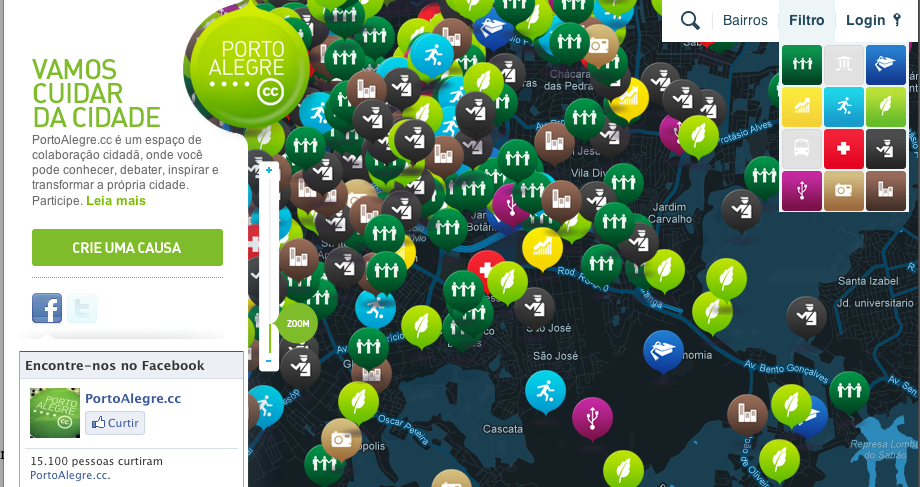
\includegraphics[scale=0.4]{portoalegre-cc}
	\end{center}
	\legend{Fonte: \citeonline{portoalegre}}
\end{figure}

Esse problema fica evidente na \autoref{fig-porto-alegre} quando consideramos, a possibilidade, que um grupo de 5 marcadores reunidos numa região específica, podem sobrepor dezenas ou até milhares de outros marcadores. Ou seja, o mapa não consegue mostrar, com clareza e precisão, as áreas de maior ocorrência de determinado incidente. 

O site fornece um filtro por categorias, que diminui de forma significativa a quantidade de informação exibida.  Mas infelizmente não resolve o problema, pois a sobreposição de informação ainda pode ocorrer com informações de uma mesma categoria.



\subsection{Zoom arbitrário}
Alguns sites criam mecanismos que minimizam o problema da sobreposição de informações. Como exemplo, temos o \citeonline{crimemapatl}  mostrado na \autoref{fig-mapatl} que mostra um mapa com a taxa de crimes em Atlanta. 

O site fornece filtros por categoria, data e zoom. Mas o principal responsável pela eliminação da sobreposição de informação é o filtro por zoom. Esse filtro agrupa todos os marcadores que estão sobrepostos, no zoom atual, em um único marcador que exibe a informação somada dos marcadores que o compõem.
 
\begin{figure}[htb]
	\caption{\label{fig-mapatl} MapATL não possui sobreposição de informação devido ao filtro por zoom}
	\begin{center}
	    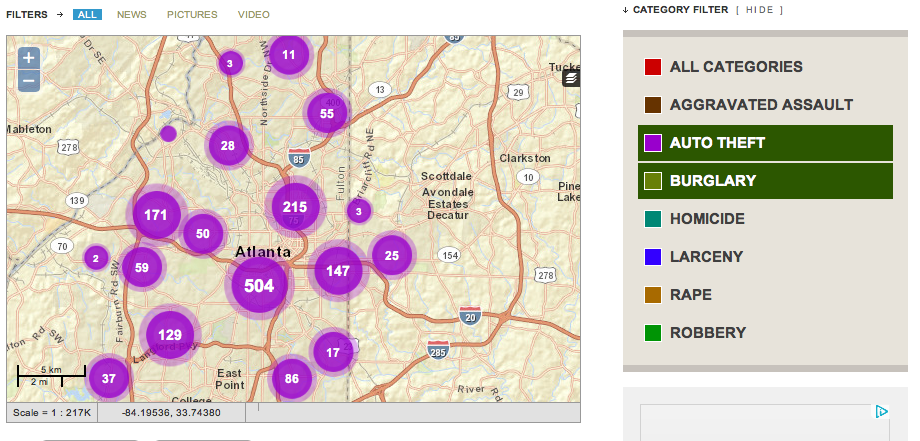
\includegraphics[scale=0.4]{crime-mapatl-com-filtro}
	\end{center}
	\legend{Fonte: \citeonline{crimemapatl}}
\end{figure}

Segundo \cite[42,44]{silva2010solap+} esse tipo de agrupamento, baseado em grelha, pode ser implementado a partir do algorítimo WaveCluster\cite{wavecluster}. 

 

\begin{figure}[htb]
	\caption{\label{fig-zoomab} Entre ZOOM A e ZOOM C existem muitos níveis intermediários e não apenas 1 (ZOOM B).}
	\begin{center}
	    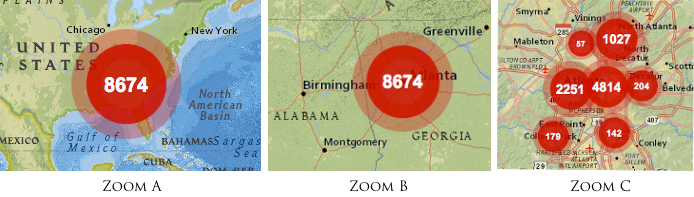
\includegraphics[scale=0.6]{zoomab}
	\end{center}
	\legend{Fonte: \citeonline{crimemapatl}}
\end{figure}

Esse algorítimo resolve o problema de sobreposição de informações. Porém o problema do zoom arbitrário permanece, ilustrado na \autoref{fig-zoomab}, permanece.

O usuário precisa aplicar vários zoons para ir do ZOOM A para o ZOOM C. Mas durante essa interação é gasto tempo e banda, da conexão deinternet, do usuário para exibir os zoons intermediários, quando o ideal seria exibir apenas o ZOOM B.

Esse gasto de banda, prejudica\footnote{dispositivos móveis que usam mapas vetoriais, como o iphone da apple, não sofrem desse problema.} a usabilidade de mapas em dispositivos móveis pois, geralmente, eles possuem pouca banda de internet.

Uma abordagem para esse problema é o uso de um zoom inteligente que siga uma hierarquia espacial invés de de simplesmente dobrar a visualização espacial. 
 





\section{Objetivos}

\section{Contribuições}

\section{Estrutura da Monografia}
